%****************************************************************************************************************************************
% File: mpm4cps-ontology.tex
%
% This file is automatically generated. Please do not edit!
%****************************************************************************************************************************************
\section{Ontology Overview}

The OWL MPM4CPS ontology that defines cross-cutting concepts between the Shared, MPM and CPS ontologies.

Figure \ref{fig:mpm_ontology_overview} shows an overview of the MPM4CPS ontology. The details of each concept are
provided in the following subsections.

\begin{figure}[!htb]
\centering
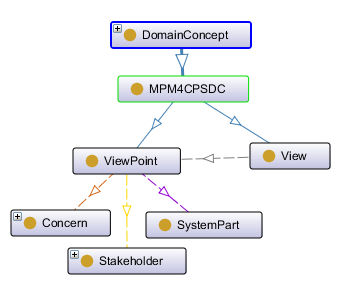
\includegraphics[width=0.5\textwidth]{figures/mpm4cps_overview.png}
\caption{Overview of the MPM4CPS ontology}
\label{fig:mpm4cps_ontology_overview}
\end{figure}



\section{Domain Concepts}

This ontology of multi-paradigm modeling contains concepts divided into sub-domains as presented in the following subsections.

\subsection{MPM4CPSDC}
\label{subsecDC:MPM4CPSDC}

MPM4CPSDC domain concept class

\subsubsection{ModelBasedEngineeringEnv}
\label{subsubsecC:ModelBasedEngineeringEnv}
\didx{ModelBasedEngineeringEnv}

In order to define our modeling paradigm notion, we first subclass the EngineeringEnvironment class of the Shared ontology by the ModelBasedEngineeringEnv class.

\textbf{Subclass of}
\begin{itemize}
	\item \textbf{MPM4CPSDC} (see section \ref{subsecDC:MPM4CPSDC})
	\item \textbf{EngineeringEnvironment} (see section \ref{subsubsecC:EngineeringEnvironment})
\end{itemize}






\subsubsection{ModelBasedProcess}
\label{subsubsecC:ModelBasedProcess}
\didx{ModelBasedProcess}

The Process class of the Shared ontology is refined into the ModelBasedProcess class to represent all processes that manipulate models instead of data fields.

\textbf{Subclass of}
\begin{itemize}
	\item \textbf{MPM4CPSDC} (see section \ref{subsecDC:MPM4CPSDC})
	\item \textbf{ModelBasedEngineeringArtifact} (see section \ref{subsubsecC:ModelBasedEngineeringArtifact})
	\item \textbf{Process} (see section \ref{subsubsecC:Process})
\end{itemize}






\subsubsection{View}
\label{subsubsecC:View}
\didx{View}

A viewpoint governs an architecture view.

\textbf{Subclass of}
\begin{itemize}
	\item \textbf{MPM4CPSDC} (see section \ref{subsecDC:MPM4CPSDC})
	\item \textbf{View} (see section \ref{subsubsecC:View})
\end{itemize}





\todoAuthors{Finally, we create another object property to relate a view to its employed models.}


\subsubsection{ViewPoint}
\label{subsubsecC:ViewPoint}
\didx{ViewPoint}

According to the IEEE 42010 standard, a viewpoint frames the concerns of stakeholders.

\textbf{Subclass of}
\begin{itemize}
	\item \textbf{MPM4CPSDC} (see section \ref{subsecDC:MPM4CPSDC})
	\item \textbf{ViewPoint} (see section \ref{subsubsecC:ViewPoint})
\end{itemize}

\section{Properties}


\subsection{hasFramedConcerns}
\label{subsecP:hasFramedConcerns}
The hasFramedConcerns object property relates a viewpoint to a set of framed concerns as defined in the Shared ontology.

Subproperty of:
None


Domains:
\begin{itemize}
	\item \textbf{ViewPoint} (see section \ref{subsubsecC:ViewPoint})
\end{itemize}


Ranges:
\begin{itemize}
	\item \textbf{Concern} (see section \ref{subsubsecC:Concern})
\end{itemize}




\subsection{hasGovernedView}
\label{subsecP:hasGovernedView}
The hasGovernedView object property relates a viewpoint to its view.

Subproperty of:
None


Domains:
\begin{itemize}
	\item \textbf{ViewPoint} (see section \ref{subsubsecC:ViewPoint})
\end{itemize}


Ranges:
\begin{itemize}
	\item \textbf{View} (see section \ref{subsubsecC:View})
\end{itemize}




\subsection{hasGoverningView}
\label{subsecP:hasGoverningView}
A viewpoint governs an architecture view.

Subproperty of:
None


Domains:
\begin{itemize}
	\item \textbf{View} (see section \ref{subsubsecC:View})
\end{itemize}


Ranges:
\begin{itemize}
	\item \textbf{ViewPoint} (see section \ref{subsubsecC:ViewPoint})
\end{itemize}




\subsection{hasStakeholders}
\label{subsecP:hasStakeholders}
The hasStakeholders  object property relates a ViewPoint to its Stakeholder.

Subproperty of:
None


Domains:
\begin{itemize}
	\item \textbf{ViewPoint} (see section \ref{subsubsecC:ViewPoint})
\end{itemize}


Ranges:
\begin{itemize}
	\item \textbf{Stakeholder} (see section \ref{subsubsecC:Stakeholder})
\end{itemize}




\subsection{hasSupportingMegamodelFragments}
\label{subsecP:hasSupportingMegamodelFragments}
The hasSupportingMegamodelFragments object property  relates a viewpoint to a set of supporting megamodel fragments.

Subproperty of:
None


Domains:
\begin{itemize}
	\item \textbf{ViewPoint} (see section \ref{subsubsecC:ViewPoint})
\end{itemize}


Ranges:
None




\subsection{hasSystemConstituentElements}
\label{subsecP:hasSystemConstituentElements}
The hasSystemConstituentElements object property relates a viewpoint with its system constituents or parts.

Subproperty of:
None


Domains:
\begin{itemize}
	\item \textbf{ViewPoint} (see section \ref{subsubsecC:ViewPoint})
\end{itemize}


Ranges:
None




\subsection{hasViewpoint}
\label{subsecP:hasViewpoint}
A set of viewpoints can be linked to a process through an object property hasViewpoint, so that data types are declared as the elements grouped under the associated megamodel fragment.

Subproperty of:
None


Domains:
\begin{itemize}
	\item \textbf{ModelBasedProcess} (see section \ref{subsubsecC:ModelBasedProcess})
\end{itemize}


Ranges:
\begin{itemize}
	\item \textbf{ViewPoint} (see section \ref{subsubsecC:ViewPoint})
\end{itemize}




\subsection{isSupportedBy}
\label{subsecP:isSupportedBy}
A ViewPoint is supported by a Formalism.

Subproperty of:
None


Domains:
\begin{itemize}
	\item \textbf{ViewPoint} (see section \ref{subsubsecC:ViewPoint})
\end{itemize}


Ranges:
\begin{itemize}
	\item \textbf{Formalism} (see section \ref{subsubsecC:Formalism})
\end{itemize}




